%!TeX root=MemoriaTFG.tex

\chapter{Arquitectura de la aplicación} \label{chapter:AppArchitecture}

En esta sección se presenta la arquitectura de la aplicación. Se realiza una 
descripción de las funcionalidades que lo componen, se definenen los requerimientos necesarios 
para su construcción y por último una explicación de la implementación, mostrando las herramientas 
usadas. El objetivo de este capítulo es mostrar al lector como está estructurada la aplicación tanto a nivel
de código desgranando las librerías externas de las que se ha hecho uso como de la solución de la 
infraestructura, apostando por una solución que facilite al individuo su uso dentro del sistema.

\section{\textit{TrackSimulator}}
\textit{TrackSimulator} es un generador pseudo-aleatorio de trayectorias geoposicionales. Se entiende como 
simulación al proceso de recrear el comportamiento, en este caso el camino de usuarios dentro de un espacio 
geográfico. Como muestra esencial y discreta del comportamiento de la población se usan registros que han 
sido obtenidos mediante localización \ac{GPS}. En la figura \ref{figure:TrackExample1} se muestra un ejemplo 
de una detección del recorrido de un individuo.
\begin{figure}[!htb]
\begin{center}
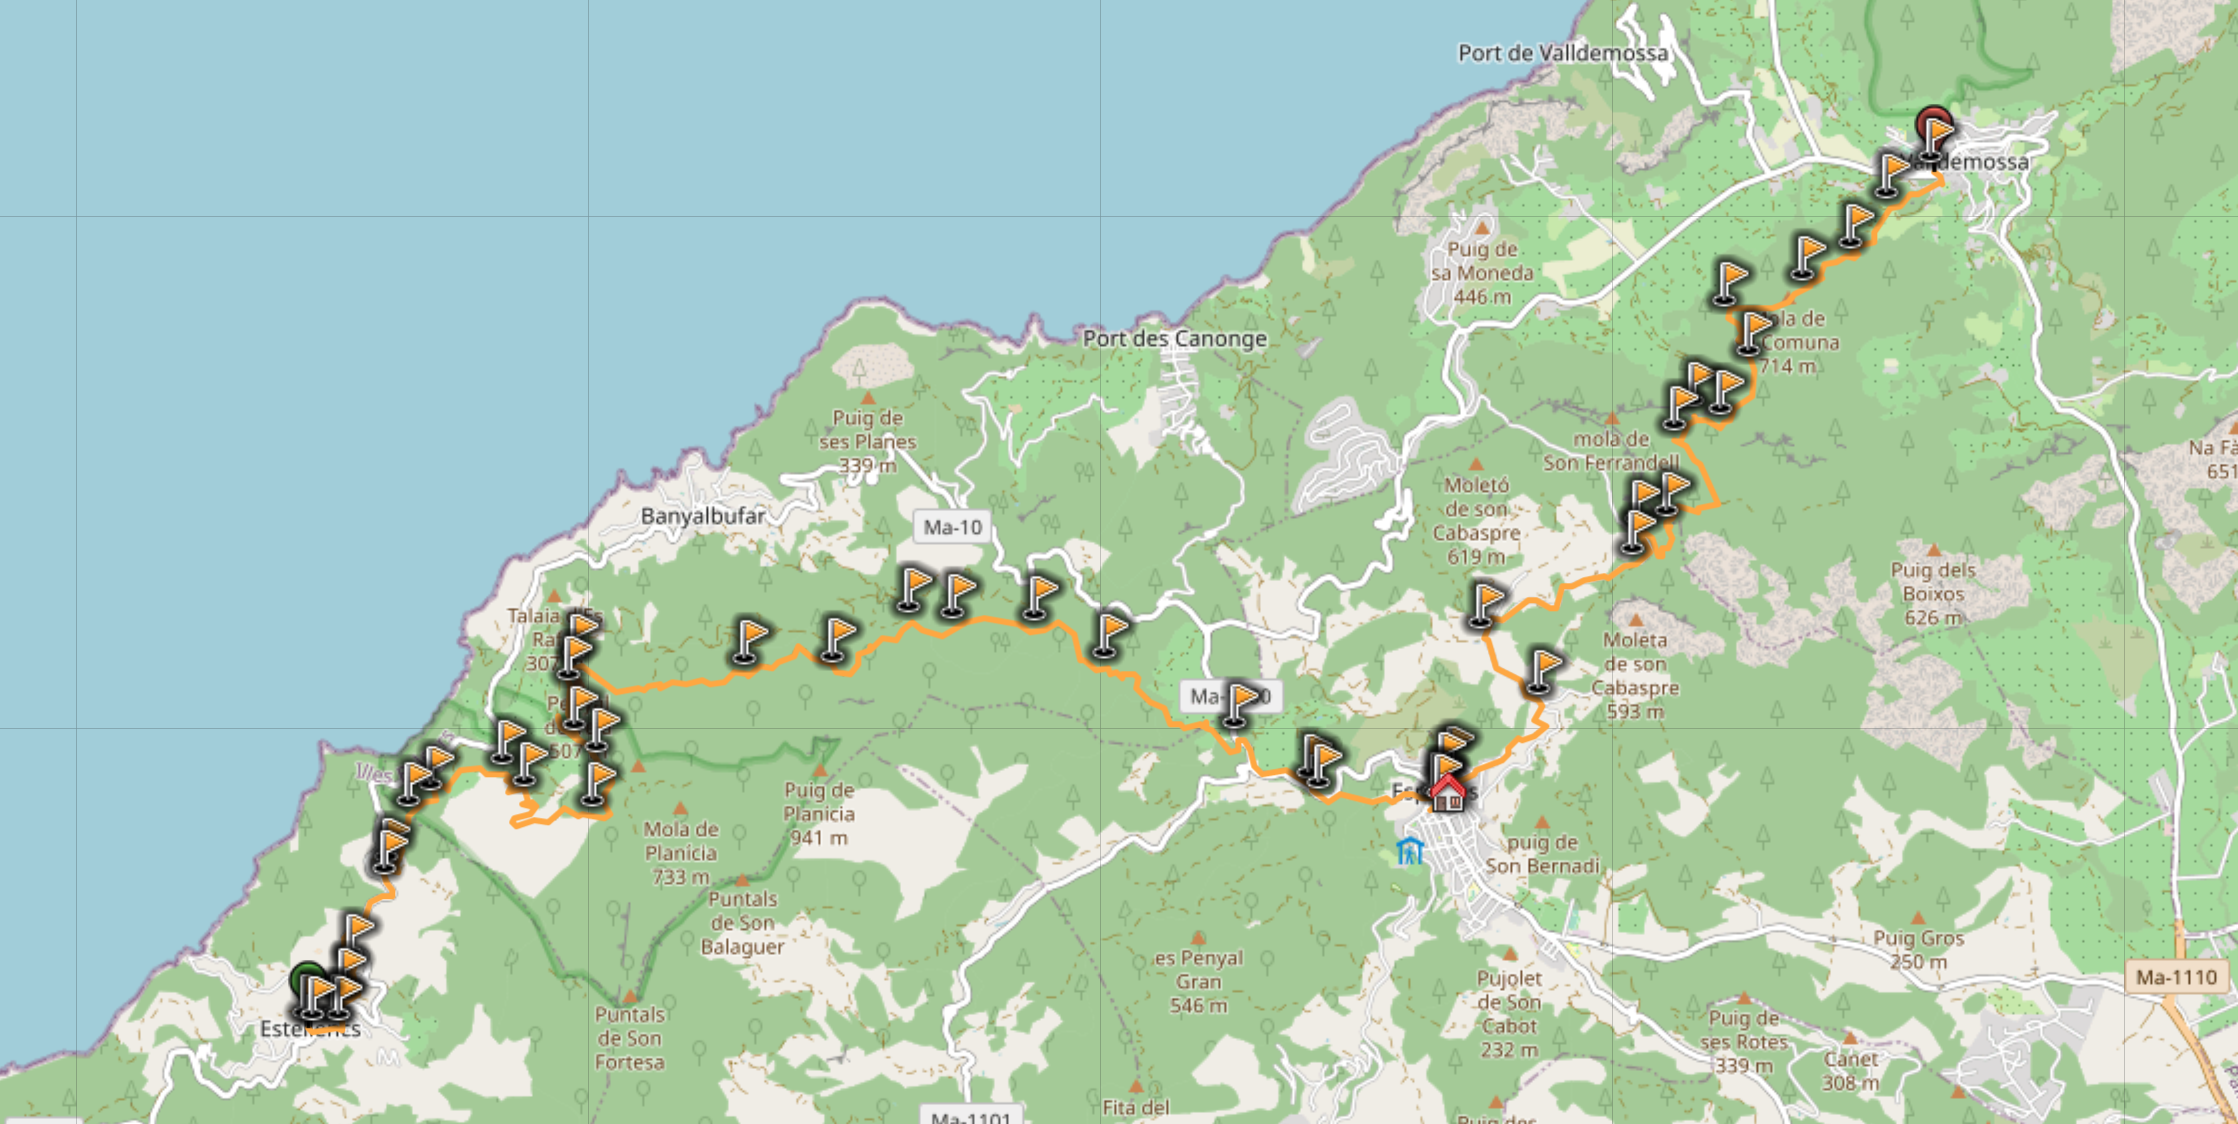
\includegraphics[width=0.5\textwidth]{./Imagenes/RealTrackDetection.png}
\caption{Ejemplo de detección real de la trayectoria de un individuo por la Serra de Tramuntana, Illes 
Balears, Mallorca, Spain}
\label{figure:TrackExample1}
\end{center}
\end{figure}
\newpage

Para realizar un algoritmo que genere trayectorias y tengan un grado de similitud con la realidad se debe 
realizar un ejercicio previo de análisis y tratamiento de información. Distancias entre las detecciones, 
desviación entre la posición de una detección del dispositivo \ac{GPS} y un camino definido son ejemplos de 
datos que se tienen que tener en cuenta para la obtención de resultados óptimos en cuanto a representación 
de la realidad.

Tanto la información muestral como la generada, así como todo el conjunto de información geoespacial debe 
ser almacenada en un tipo de estructura lógica que permita el acceso y manipulación de estos de la forma 
más eficiente posible. 

Teniendo una estructura lógica que permita almacenar la información, el problema determinante será la 
forma en la que los datos geoposicionales, en este caso puntos \ac{GPS} pasan a formar parte de esté 
modelo. Recordemos que un punto \ac{GPS} contiene únicamente información de la posición dentro de la
superficie terrestre, no obstante no aporta información de la asignación de este punto a un segmento de
un camino, calle, o paraje concreto. La asociación de un punto \ac{GPS} a un tipo vía es un problema conocido 
con el nombre de \textit{Map matching} y la propuesta de este documento a su resolución se realizará en 
detalle en el apartado \ref{section: MapMatching}.

Con la estructura lógica y la información integrada en ella, el análisis de la información permitirá tomar 
el conjunto de decisiones que permitan maximizar el grado de exactitud de la simulación para, 
posteriormente, realizar el algoritmo que permita realizar dicha recreación. La transformación del dato desde una trayectoria real hasta la generación final de trayectorias simuladas queda ilustrada en la figura \ref{figure:TrackSimulatorDiagram}.
\begin{figure}[!htb]
\begin{center}
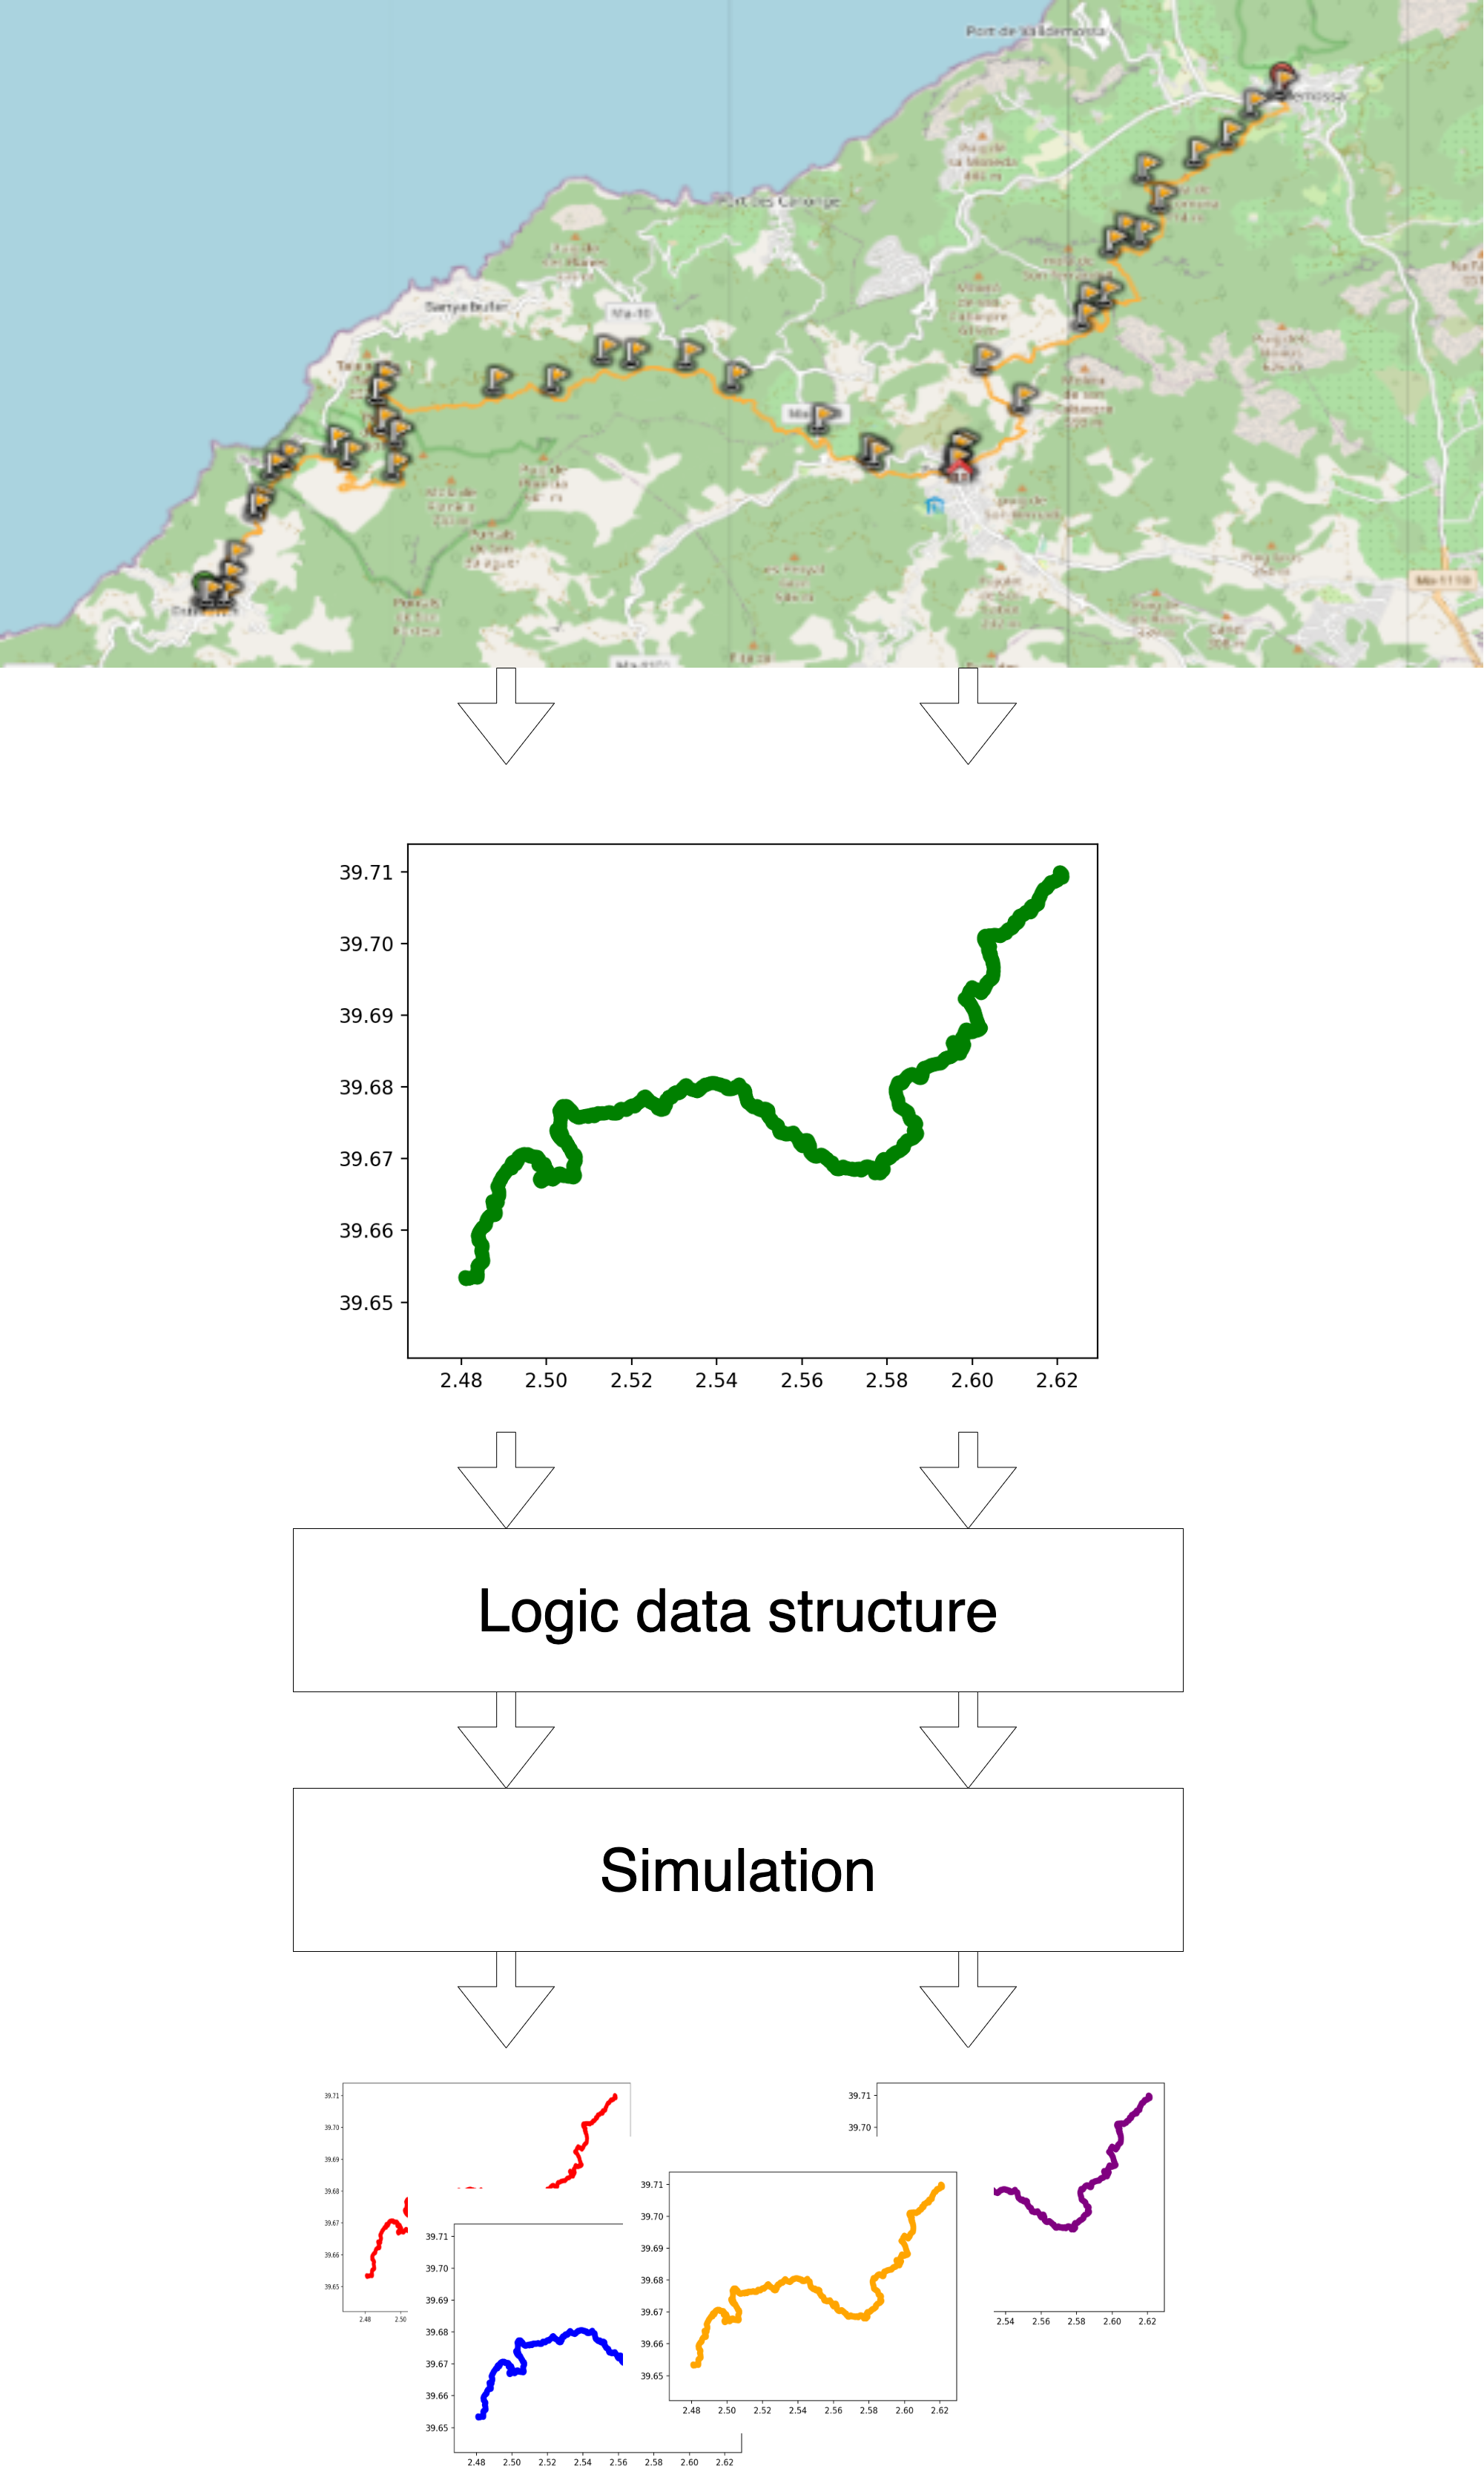
\includegraphics[width=0.5\textwidth]{./Imagenes/TrackSimulatorStructure.png}
\caption{Diagrama de funcionamiento de TrackSimulator}
\label{figure:TrackSimulatorDiagram}
\end{center}
\end{figure}
\newpage
 
La aplicación crea una sucesión de puntos que equivalen a un recorrido dentro de un plano geográfico. 
Se ha determinado que la generación de puntos dentro del aplicativo se realiza de forma pseudo-aleatoria, quiere decir que la producción de los diferentes puntos no sigue ningún patrón o regularidad en sí misma sino que parte del análisis realizado, al que se le añaden componentes aleatorios. La sucesión de puntos estará relacionada directamente con un camino, sendero o recorrido asignado al modelo lógico. La simulación tendrá en cuenta la frecuencia de paso relativa por el segmento como parte del proceso, así como la distancia entre los puntos uno a uno. Con este procedimiento se pretende obtener de una forma rigurosa un análisis cuantitativo de los datos aportados por las trayectorias reales para poder crear una simulación lo más real posible.

\section{Funcionalidades de \textit{TrackSimulator}}
\textit{TrackSimulator} es una aplicación. El término \textit{aplicación} se entiende como la suma de 
conjunto de implementaciones  de código ejecutable y del que se espera un resultado. El flujo del aplicativo se puede ver en la figura red \ref{figure:TrackSimulatorDiagramFlow}. Consta de un único tipo de entrada, en este caso trayectorias sobre un terreno en ficheros \ac{GPX}. Los dos grandes módulos representan el análisis y la simulación de los datos, donde en el primero realizará una alimentación de una base de datos con la información de las trayectorias y el resultado del análisis, por otra parte almacenará en la máquina una imagen del resultado del análisis. El módulo de simulación realizará el proceso de generación de trayectorias a partir de la lectura de los datos almacenados en la base de datos, del que también se obtienen imágenes de las trayectorias.

\begin{figure}[!htb]
\begin{center}
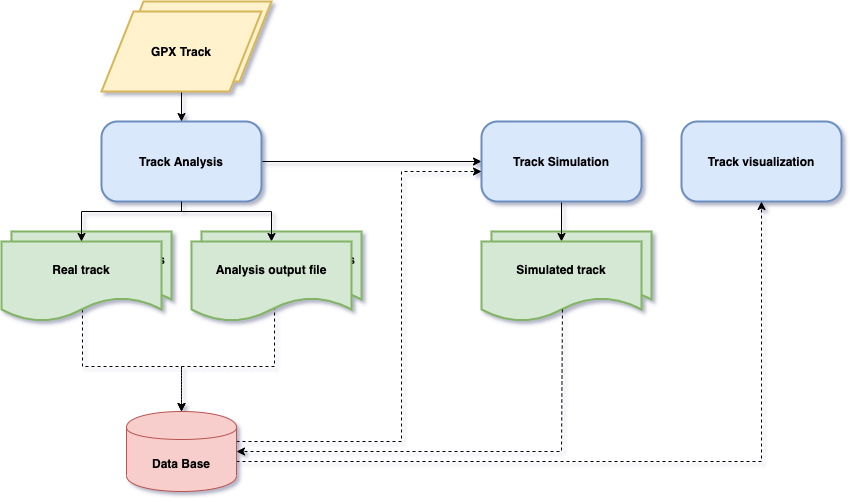
\includegraphics[width=0.99\textwidth]{./Imagenes/TrackSimulatorDiagram.png}
\caption{Diagrama de funcionamiento de TrackSimulator}
\label{figure:TrackSimulatorDiagramFlow}
\end{center}
\end{figure}

La aplicación recopila la siguiente serie de funcionalidades:
\begin{description}
\item [Importación y análisis de archivos \ac{GPX}] La aplicación soportará la importación de un archivo GPX concreto, o bien de un conjunto de archivos GPX. Estos archivos GPX deben contener trayectorias realizadas en el espacio delimitado. La funcionalidad del aplicativo se basa en un territorio acotado, por lo que el conjunto de rutas a analizar deben corresponder con el territorio especifico para que el proceso de análisis 
se complete. 

La aplicación, con los datos importados por los archivos, permitirá un análisis de trayectorias aplicando técnicas de \textit{map matching}. Del análisis se obtendrá información:
\begin{description} 
\item[Distancia entre puntos]  Distancia entre las capturas de posición \ac{GPS} en el fichero punto a punto.
\item[Distancia relativa entre punto de ruta y punto de trayectoria] Distancia del punto \ac{GPS} detectado 
de la trayectoria la punto proyección dentro de la ruta, camino o vía seleccionada como más probable en el proceso de\textit{map-matching}.
\item[Frecuencia de paso por segmento de ruta] Frecuencia de paso por el segmento $x_{a}, x_{b}$ relativo 
a todos los segmentos desde $x_{a}$.
\end{description}
El detalle de esta información se describe en detalle en el capítulo \ref{section:ExplotacionDato}. Toda esta información quedará almacenada en una base de datos de forma que la información sea accesible para realizar la simulación de la ruta.
\item [Muestra de resultados del análisis] La aplicación permite la representación gráfica de información gráfica de los resultados del análisis. Las  imágenes serán almacenadas en formato \ac{PNG}.
\item [Creación de una trayectoria a partir de parámetros y exportación \ac{GPX}] Con los resultados de la información analizada se puede realizar una simulación de trayectorias dentro del espacio geográfico delimitado. Los parámetros a introducir quedan detallados en el capítulo \ref{chapter:GuiaUso}. Estas trayectorias quedarán representadas en formato \ac{GPX}. 
\item [Visualización de la trayectoria] La aplicación mostrará una representación gráfica de la trayectoria tanto   dentro del territorio geográfico a partir del almacenamiento de imágenes en formato  \ac{PNG}.
\end{description}


\section{Requerimientos de \textit{TrackSimulator}} \label{section: RequerimientosTrackSimulator}
Explicadas las funcionalidades de la aplicación de Track Analyzer los requerimientos identificados son los siguientes:
\begin{enumerate}[label={R.\arabic*.}]

\item \textbf{Importación de datos} La aplicación debe realizar una importación de los datos desde un fichero .\ac{GPX} al modelo lógico elegido para la el posterior tratamiento.

\item \textbf{Análisis de trayectoria} La aplicación debe realizar un análisis de la trayectoria que proporcione por una parte indicadores y por otro valores medibles, cuantificables y utilizables para realizar una simulación 
lo más precisa posible.

\item \textbf{Almacenamiento de las rutas reales en base de datos} La aplicación debe realizar un almacenamiento de los datos analizados en una base de datos, con el objetivo de poder ser repetible
sin necesidad de importar nuevamente los datos.

\item \textbf{Almacenamiento del análisis en base de datos} La aplicación debe realizar un almacenamiento de los resultados del análisis en una base de datos, con el objetivo de poder ser accesibles para la
etapa de simulación.

\item \textbf{Generación de fichero de gráficas resultantes del análisis}  La aplicación debe poder realizar una muestra de la información resultante para su visualización por parte del usuario.

\item \textbf{Lectura de la base de datos para el acceso a la información} La aplicación debe poder realizar una lectura de la base de datos para acceder a la información necesaria para la muestra de resultados o 
simulación de trayectorias.

\item \textbf{Simulación de puntos \ac{GPS} a partir de resultado de análisis} La aplicación debe poder generar el camino más probable dada un análisis previo y unos parámetros de entrada. La aplicación debe generar los puntos de cada uno de los segmentos necesarios dado un camino.

\item \textbf{Generación del fichero GPX correspondiente a la simulación de la trayectoria}  La aplicación realizar una exportación de los datos a formato .\ac{GPX}.

\item \textbf{Generación de fichero visualización de trayectoria}  La aplicación debe poder mostrar al usuario una visualización de la trayectoria dado un fichero .\ac{GPX}.

\end{enumerate}

\section{Implementación de TrackSimulation}
\subsection{Flujo de datos}

\begin{figure}[htb]
\begin{center}
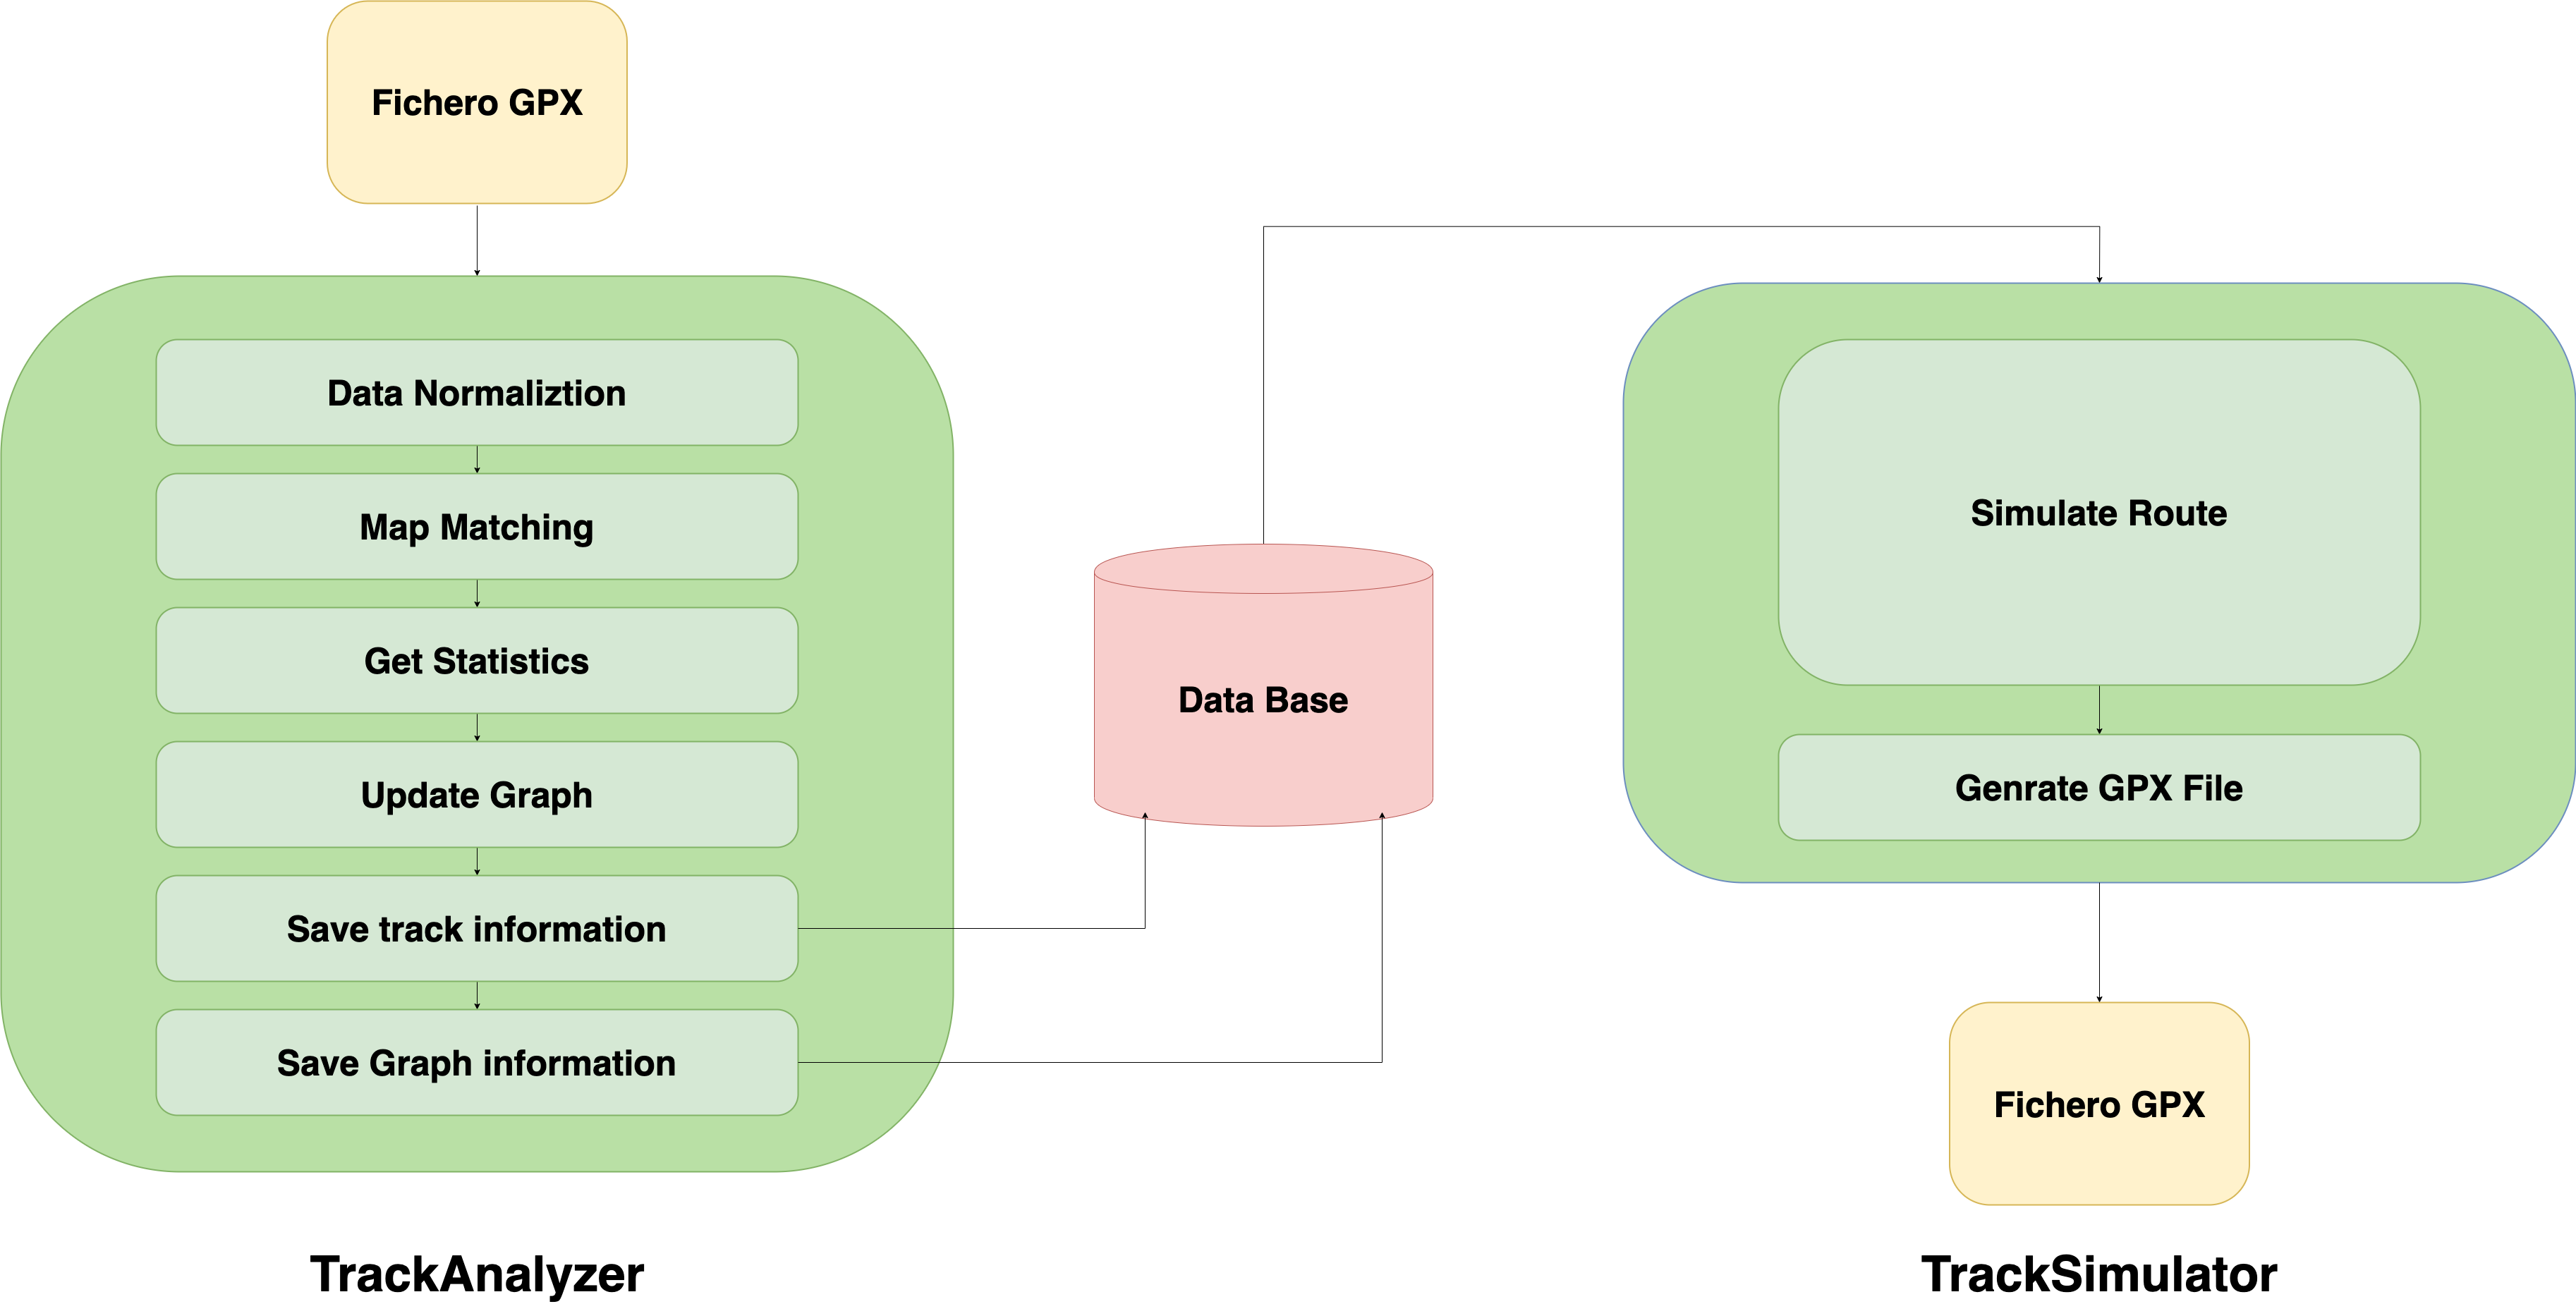
\includegraphics[width=0.9\textwidth]{./Imagenes/TrackSimulatorDataFlow.png}
\caption{Flujo de datos de TrackSimulator}
\label{TrackSimulatorDataFlow}
\end{center}
\end{figure}

Podemos ver en la figura \ref{TrackSimulatorDataFlow} de la parte superior la implementación de la aplicación 
dos grandes módulos. Por una parte encontramos \textit{TrackAnalyzer}. Este módulo es el encargado de 
realizar todas los procesos de tratamiento de datos para su posterior análisis. Inicialmente en el alcance de 
este proyecto se realizará análisis de ficheros \ac{GPX} por lo que es el único modelo de datos que entrará en 
nuestro sistema. Para realizar un análisis se realiza un proceso de tratamiento previo de datos, que se detalla 
en el apartado \ref{section: ImportacionGPX}.

Posterior al tratamiento de datos se realizará el proceso de \textit{Map Matching} con el que se une los datos 
introducidos al modelo lógico del territorio geográfico. El proceso de \textit{Map Matching} queda descrito 
en detalle en el apartado \ref{section: MapMatching}.

Una vez se ha realizado la asignación por cada punto a un camino determinado se puede realizar un análisis 
del fichero, del cual se obtienen las métricas requeridas por el apartado 
\ref{section: RequerimientosTrackSimulator}. La descripción de la forma en la que se explotan los datos está
detallada en la sección \ref{section:ExplotacionDato}.

Con la explotación del dato hecha, únicamente queda guardar la información generada en una base de datos.
El almacenamiento de las trayectorias analizadas y mapeadas, el resultado de los análisis y la estructura 
lógica con la información modificada se realizarán de forma independiente en secciones diferentes de la 
base de datos.

El módulo de \textit{TrackSimulator} tiene la responsabilidad de generar la simulación de una trayectoria 
a partir de unos parámetros de entrada. Una vez generada la simulación, un fichero \ac{GPX} con las 
coordenadas será el producto final del proceso.
 
\subsection{Herramientas externas utilizadas} 
Como herramientas externas utilizadas para la realizar la propuesta de este documento se destacan 
el tipo de almacenamiento de datos que se utilizarán, así como las librerías externas que se han usado 
para la implementación de la aplicación. A continuación se detallan ambas.

\subsubsection{Almacenamiento del dato}
Tanto de trayectorias reales como de los datos generados por el análisis deben ser almacenados 
de forma que sean accessibles de forma rápida.
Para el almacenamiento de datos, existen dos grandes posibilidades: el uso de Bases de datos relacionales, 
a partir de ahora descritas como \ac{SQLDB},
o el opuesto, las bases de datos no relacionales, \ac{NOSQLDB}.
Para la realización de la propuesta descrita en este documento se ha decidido realizar el almacenamiento de 
toda la información en \textit{MongoDB}, una de las \ac{NOSQLDB}
más usadas y que detallamos a continuación.

\textit{MongoDB} se trata de una \ac{NOSQLDB} de código abierto y su funcionamiento es documental. 
Se almacenan colecciones de documentos, que son series de elementos clave-valor en formato JSON.

MongoDB elimina las limitaciones de las bases de datos relacionales \cite{Mongo01}. 
Permite almacenar de forma eficiente grandes cantidades de información, siendo
a su vez flexible a modificaciones debido a que los documentos que se almacenan en las colecciones no tienen 
una taxonomía definida. Por lo que el desarrollo incremental de la aplicación y la aparición de nuevos 
campos dentro del modelo de datos no es un problema.
Otro gran motivo para la elección de MongoDB como base de datos de este proyecto es la escalabilidad 
que ofrece, de forma que a grandes cantidades de trayectorias por almacenar, podría distribuirse utilizando servicios en la nube.

Actualmente para el desarrollo de la propuesta no se ha contado con una gran cantidad de datos.
No obstante el problema ha sido planteado con el objetivo de poder analizar grandes cantidades de datos y que puedan
ser almacenados y accesible mediante el uso de esta base de datos.

\subsubsection{Librerías utilizadas} \label{subsection: LibreriasExternas}
El lenguaje seleccionado para el desarrollo del aplicativo ha sido Python debido al ser recomendable para el tratamiento de datos. Su flexibilidad y la gran utilidad aportada por librerías externas hacen que sea idóneo para el desarrollo de la propuesta. Entendemos como librería un conjunto de código agrupado que aporta funcionalidad diversa. Las librerías externas empleadas en este proyecto son las siguientes :
\begin{enumerate}[label={L.\arabic*.}]
%gpxpy
\item \textbf{gpxpy} Librería para la manipulación de ficheros \ac{GPX}. Mediante esta librería se puede realizar una importación del fichero para su posterior manipulación. De esta forma se obtiene la secuencia de puntos \ac{GPS} que describe una trayectoria determinada.
%pandas
\item \textbf{pandas} Librería para el análisis de los datos. Toda la información correspondiente a las diferentes trayectorias queda reflejada en un Dataframe para su posterior tratamiento y acceso.
%osmnx
\item \textbf{osmnx} Librería para la extracción, visualización y análisis de redes de calles. Mediante esta librería se puede obtener toda la información referente a nuestro espacio determinado del Castillo de Bellver e importar toda la información de sus caminos y carreteras transitables. De esta forma tenemos toda una estructura de datos con información geográfica precisa del entorno. Por otra parte mediante esta librería se puede visualizar las trayectorias escogidas, así como la capacidad de almacenar imágenes de las trayectorias analizadas o simuladas.
%matplotlib
\item \textbf{matplotlib} Librería por excelencia para la representación de información de forma visual. Mediante el uso de esta librería podemos mostrar diversas gráficas de la información obtenida y analizada por los diferentes algoritmos.
%numpy
\item \textbf{numpy} Librería para el cálculo científico. Esta librería nos aporta diferentes estructuras de datos para el acceso y cálculo de forma eficiente a la información. Una de las principales ventajas de esta librería es la implementación de matrices de forma que el acceso a los datos incrementa su eficiencia de forma considerable.
%geopy
\item \textbf{geopy} Librería para el tratamiento de coordenadas. Mediante esta librería se obtienen las herramientas necesarias para tratar al par de datos \textit{(Lat,Long)} como un punto de coordenada  \ac{GPS}. Por otra parte se obtiene implementación del cálculo de la distancia entre dos coordenadas.
%itertools
\item \textbf{itertools} Esta librería implementa diversos bloques de iteradores. El uso dentro de nuestro proyecto queda exclusivamente para la agrupación de elementos dentro de un set de datos.
%sklearn
\item \textbf{sklearn} Librería para el análisis de de datos. Esta librería nos aporta todas las herramientas necesarias para el análisis de los datos \ac{GPS}. Con ella realizamos los cálculos de puntos próximos a partir de una búsqueda basada en \ac{BSP} como veremos en la siguiente sección.
%shapely
\item \textbf{shapely} Librería para el tratamiento de figuras geométricas. De esta forma podemos tratar elementos comos puntos \ac{GPS} de forma abstracta. Por otra parte nos permite tratar las rutas del espacio a analizar como una linea de sucesivos puntos \ac{GPS}.
%pickle
\item \textbf{pickle} Librería para la codificación-decodificación de ficheros. Mediante el uso de esta librería se realiza la exportación de la información estadística y de la estructura de grafo generada y almacenada en los ficheros .txt/edgelist sucesivamente.
\end{enumerate}

\subsection{Docker}
Para poder entender completamente este apartado tenemos que hacer una mención a la forma clásica de arquitectura de 
proyectos software a nivel de infraestructura. Esta forma tenía como particularidad el uso de máquinas virtuales para la 
ejecución de las diferentes aplicaciones, así como un supervisor de las máquinas virtuales.  Cada máquina virtual desplega
su propio sistema operativo con sus dependencias. Por otro lado, encontramos la forma mediante el uso de contenedores.

Una de las implementación más usada de contenedores es Docker. Docker es una plataforma para el desarrollo, despliegue y ejecución de aplicaciones basado en contenedores \cite{Docker01}.  Una imagen es 
una plantilla de lectura donde está almacenado todo el código (normalmente compilado) junto con todas las dependencias 
necesarias para que pueda ser ejecutado completamente. Un contenedor es una instancia de una imagen, esta puede creada, 
desplazable y parada a partir de la \ac{API} de Docker.

\begin{figure}[!htb]
\begin{center}
\includegraphics[width=0.9\textwidth]{./Imagenes/DockerComparision.png}
\caption{Comparación entre arquitectura Docker y mediante máquinas virtuales. \cite{Docker02}}
\label{DockerComparision}
\end{center}
\end{figure}


Con esta nueva forma, todas las aplicaciones comparten el mismo sistema operativo, no es necesario ningún supervisor 
y la responsabilidad de las dependencias queda localizada en los contenedores, que contienen únicamente lo necesario 
para poder ejecutar la aplicación.

La ejecución del aplicativo tiene como requerimientos una serie de dependencias, que la máquina física puede tener o no 
en su sistema. Para añadir una capa de abstracción a la arquitectura y hacerlo replicable y desplegable en cualquier máquina
se ha utilizado Docker. La ventaja de usar Docker en esta propuesta reside en la capacidad de la plataforma de usar los 
recursos del sistema de forma eficiente, así como la portabilidad que ofrece.

La infraestructura la propuesta es la siguiente:
\begin{figure}[htb]
\begin{center}
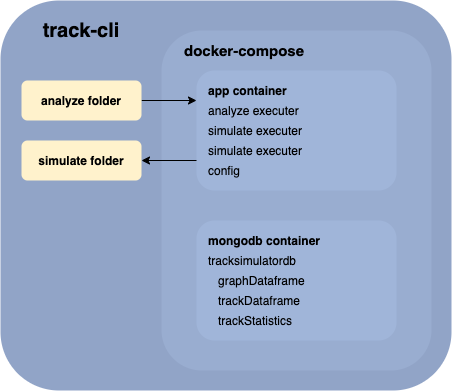
\includegraphics[width=0.8\textwidth]{./Imagenes/DockerStructure.png}
\caption{Infraestructura de la propuesta de TrackSimulator}
\label{DockerComparision}
\end{center}
\end{figure}
\newpage

Como vemos la aplicación constará de un \ac{CLI} que se encargará de centralizar todo el aplicativo. 
Mediante comandos se podrá realizar cada una de las acciones de la aplicación. Es este \ac{CLI} el 
encargado de desplegar los contenedores tanto de la base de datos como de la aplicación. Añade 
una serie de directorios que serán el puente de comunicación entre la aplicación y la máquina que lo 
ejecuta. En una carpeta se añadirán los ficheros \ac{GPX} a analizar, y como salida de la simulación 
tendremos ficheros \ac{GPX} e imágenes de la ruta en formato PNG.


